\documentclass[11 pt,letterpaper]{article}
\usepackage[margin=0.85 in]{geometry}
\usepackage{amsmath,graphicx,booktabs,array,url}
\usepackage[hidelinks]{hyperref}
\setlength{\emergencystretch}{1em}
\title{Supplementary Material\\Gate-Aware Budgeted NDT Recovery for Prior-Map LiDAR--Inertial Localization}
\author{[Author names pending approval]}
\date{Advisor-review version, October 24, 2026}
\begin{document}\maketitle
\section{Scope and Experiment Lineage}
This supplement preserves protocol distinctions and material negative evidence while the main article concentrates on the retained observation path. No new registration, data preparation, parameter tuning, or reference-error experiment was performed to prepare the submission package. All reported values come from frozen research records.

\begin{table}[h]\centering\small
\begin{tabular}{p{0.17\textwidth}p{0.31\textwidth}p{0.42\textwidth}}
\toprule
Archive cohort & Input / state predictor & Evidence and limitation\\\midrule
P45 & Matched 300 scans; original IMU/EKF and local tiles & Target-memory trade-off, no live tile crossing; not the recovery-window footprint.\\
R19 & Two 60-scan windows, four initializations; optimizer-only pose-history predictor & 480 native outputs plus 6 stability calls; distinct terminal neighborhoods, not a strict local-minimum proof.\\
R20--R21 & Same development windows, normal/+8 deg initialization; pose-history predictor & Gate/multistart/relative admission mechanisms; cannot substitute for true IMU closure.\\
R22 & Four predefined new 60-scan windows; frozen relative-only rule & Normal-initialization counterexample; not a holdout validation of later C+G.\\
R23--R24 & True IMU, deskew and delayed EKF; W 1/W 3 & Original and C+G causal histories; geometry and freshness modes separated.\\
R25 & One independent W 1/C 3 G-only 60-scan run & Same post-quality rule,60 nominal alignments, zero retries; actual output equals original.\\
R26--R27 & Literature/protocol extraction and manuscript preparation & No new estimator run. Public comparison is contextual rather than a same-protocol ranking.\\
\bottomrule
\end{tabular}
\end{table}

\section{Initialization, Reference, and Time Contract}
For $T_{A,B}$ mapping $B$ coordinates into $A$, the single archived convention interprets the CSV pose as $T_{M,B}$ and composes
\begin{equation}
T_{M,L}=T_{M,B}T_{B,C}T_{C,I}T_{I,L}.
\end{equation}
$C$ denotes left-camera optical axes, $I$ the Ouster IMU, and $L$ the point-cloud frame. Base and optical axes are not set equal. Numeric transforms, original calibration files and direction checks are retained in the conditional Base pilot archive. Paper/robot-model support establishes the preregistered assumption; it does not supply a direct certification of the local CSV export. The official reference documentation distinguishes RS\_C 1 for the Stereo-Cam setup from Base for the Multi-Cam setup. No later error-driven alignment or frame switch was introduced.

The principal ablation uses raw 2600 for one-time reference initialization, then raw 2601--2660 for evaluation. Map-axis yaw+8 degrees changes the complete initialized lidar/IMU chain consistently. Zero velocity/bias initialization is an inherited prior, not a stationary calibration measurement. Subsequent current/future reference poses do not generate online predictions. W 3 uses raw 6500 as anchor and raw 6501--6560 as evaluation.

Integer scan stamps, original relative point times and real IMU measurements are retained. The inherited adapter and deskew reference scan start. NDT observations keep that measurement time; fusion uses historical update and IMU replay rather than applying the result blindly at computation completion. Native outputs and decisions were sealed before reference evaluation. The reference interpolation gap cap is 150 ms with a 50 ms near-endpoint limit; no time offset is fitted. The fused state is evaluated at its actual recorded propagated time, not at a different earlier scan stamp.

\section{Quality and Budget Details}
Sixteen azimuth sectors define eight potential odd-sector blocks. Activity requires at least ten original input points per block, at least four active blocks and 300 even-sector points. The same active set is used for every candidate. Full NDT uses the points scored by Coverage Consistency Mean; this is not independent held-out evidence.

Each recovery event allows two native Full calls from fixed map-yaw+5/-5 degree initializations, with unchanged translation. Every candidate faces the same finite/converged/coverage/overlap/mean checks. No acceptable candidate means no map observation, with real inertial propagation continuing. The approved per 60 scan quota is 12 extra calls; it is not an indefinite online scheduler. Native transformation probability is maximized; exact ties use a distance normalized by 0.8 m/5 degrees and then candidate ID. Those normalizers are not candidate-to-prediction hard admission limits. The existing adjacent-observation publication limiter and EKF update limits remain distinct.

\begin{figure}[h]\centering
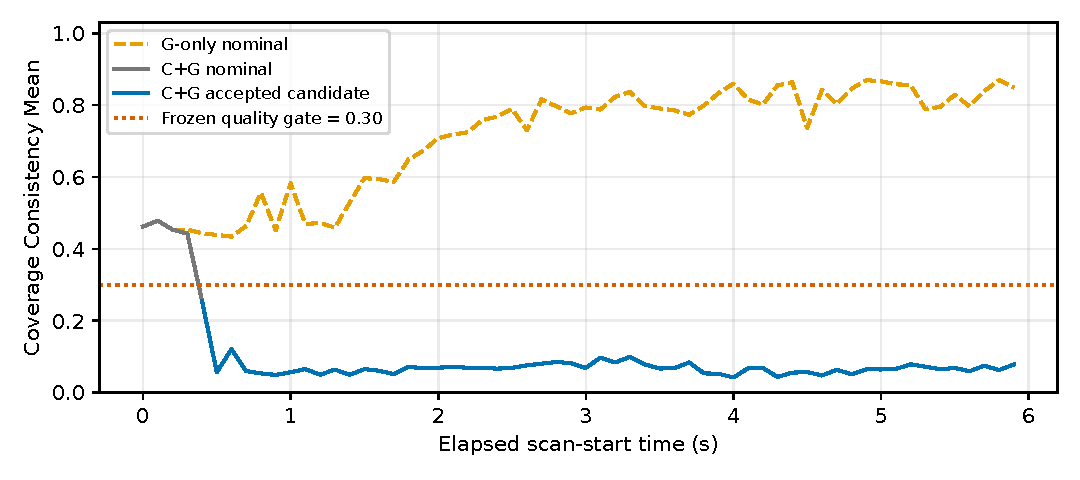
\includegraphics[width=0.86\textwidth]{figures/coverage_admission.pdf}
\caption{Frozen W 1/C 3 quality decisions. A missing selected value denotes no admitted map observation, not zero loss. The constant 0.30 threshold was not tuned using the G-only ablation. This plot is a consistency/admission diagnostic rather than independent correctness evidence.}
\end{figure}

\section{Material Counterexamples and Excluded Mechanisms}
In the optimizer-only experiment, the disturbed strong-window trajectory has position RMSE of 0.947759 m and rotation RMSE of 7.788894 degrees. Normal initialization gives 0.159179 m and 2.033813 degrees, respectively. Six repeated native optimizations remain within 0.031275 m/0.197372 degrees of their terminal neighborhoods. The harmful branch has abnormal native scores and coverage. The hypothesis of harmful convergence with a competitive native score is therefore not established. The developed 0.30 quality gate flags 21 suspect records plus 14 other records among 480 original outputs. These are exploratory counts, not independently labeled detection rates.

With a historical pose-only predictor, gate-only damages the weak-window disturbed trajectory (4.164507 m/7.016976 degrees) while simple multistart yields 0.266655 m/1.862490 degrees. In the strong window, multistart and gate-only coincide at 0.351154 m/4.143002 degrees and fail the joint development target. These results motivate distinguishing rejection from recovery, but they are not the real-IMU ablation in the main paper.

An explored relative-only rule improves a strong development case, but its frozen holdout comparison exposes normal-initialization harm: simple multistart gives 0.211401 m/2.422765 degrees, while relative admission gives 0.242043 m/2.620034 degrees and increases high-error outputs from 2 to 5. The position increase 0.030641 m exceeds its prespecified 0.03 m boundary. A favorable disturbed-initialization result cannot erase that counterexample. Relative-only admission and two-frame confirmation are excluded from C+G.

An OOSM-history synchronization trial receives 415 corrected messages and replaces 4 exact-time latest samples, but zero later NDT queries consume a replaced sample. The legal replacement samples are later than the next scan start and correctly excluded. No benefit is attributed to this switch; it is not part of the retained method. Coupled-subspace experiments are likewise not included as positive contribution evidence.

\section{Resource Scope and Deployment Status}
The matched map study uses global target 3,142,751 points versus 552,716 active points in 21 tiles. Process high-water memory 775,308 versus 138,200 KiB gives 82.2 percent reduction. Steady align mean grows 7.086 to 8.079 ms, position maximum 0.119675 to 0.216396 m, and rotationRMSE 1.81802 to 1.87495 degrees. Live tile replacement is not exercised; a separate map-replacement probe uses a real point cloud and a synthetic pose with zero NDT calls. These profiles are not an identical-binary kernel benchmark.

The recovery ablation instead uses 2,297,615 target points. Recent per-process and simultaneous pair RSS are sampled every 50 ms and exclude publisher, external deskew, visualization and the rest of the machine. Callback maxima include initialization. No whole-system 82.2 percent or 10 Hz guarantee is claimed. Some archived hardware metadata remain unreported; a current CPU model is not retrospective evidence.

Robot loop 2 assets are present, including a 19.68 GB bag,10,905 lidar scans and 218,101 IMU messages with a matching FAST-LIVO 2 map. However, its historical identity/zero lidar--IMU transform is explicitly a fallback assumption, not verified physical calibration. No new robot baseline/C+G run was performed; the 0.30 threshold is not validated across these sensor/quality scales. Existing same-system mapping poses would not be independent physical truth.

\section{Published Results and Artifact Availability}
The original Short sequence is identified by the official 1530 s OS 1 description, paper length about 1609 m and exact 15301 public-trajectory timestamp matches. Published odometry ATE and direct-map localization remain different tasks. DLIO's 0.3606 m is printed as 0.360 m in the later 2 Fast comparison; no reason for the precision difference is invented. FAST-LIO 2 and DLIO values in 2 Fast are copied from Chen 2023, and STEAM-LIO from Burnett 2025. Chen omits the first 100 FAST-LIO 2 poses for some sequences; the affected list is not reported. Short rotation RMSE is absent in the relevant tables.

The inspected 2 Fast author manuscript is arXiv2410.05433v3: Table 7 p 18, computational Table 12 p 21. Full publisher retrieval was blocked; byte identity with the version of record is not asserted. STEAM author Table II, p. 10 and Singer publisher Table III, printed p. 698 supply their original values. Public STEAM/Singer files have valid times and TUM schema, but neither a certified map transform/body-frame binding to this study nor a matching disturbed initialization. No fitted transform is used to generate new comparable scores.

The full literature extraction and all frozen experiment paths are mapped in the accompanying evidence ledger. \textbf{[Authors must approve the final public release URL/DOI and permissions before submission.]}
\end{document}
